\chapter{Python for Data Science} \label{ch:python}

Python is has been increasingly popular for data science. Many libraries and tools have been developed delicately for Python to enhance its data analysis and visualization capability, such as \verb|numpy|, \verb|scipy|, \verb|scikit-learn|, \verb|pandas|, \verb|matplotlib| \verb|tensorflow| and \verb|pytorch|, just to name a few.

This chapter introduces commonly used tools and approaches that data science adopt using Python. This part of the notebook is more application driven, and only the basic implementations are introduced. We are not digging into the theory supporting machine learning and artificial intelligence.

It has been increasingly popular today, to use Python together with Conda and jupyter notebook. Conda is an open-source language-agnostic package and environment management system. Jupyter notebook is an interactive computing platform for Python and other computer programming languages. The detailed introduction to the installation and usage of Conda and Jupyter notebook is not covered here. They are used when demonstrating the examples in this chapter.

\section{Introduction to \texttt{pandas} Package}

The \verb|pandas| package is a widely used powerful data processing toolkit. With \verb|pandas|, Python gains the ability to handle data frames like Microsoft Excel. Some of the features and functions of \verb|pandas| are worth introducing separately before hand, hence this section.

This is not to say that other packages are less important or less complicated by all means. Some of these packages work together with \verb|pandas| to process data, while others may have their own ways to handle data frames. It is just that \verb|pandas| is a fundamental package that can be introduced stand alone.

Assume that \verb|pandas| is correctly installed in the machine, and a jupyter is opened as shown in Fig. \ref{ch:python:fig:jupyter_cover}.

\begin{figure}
	\centering
	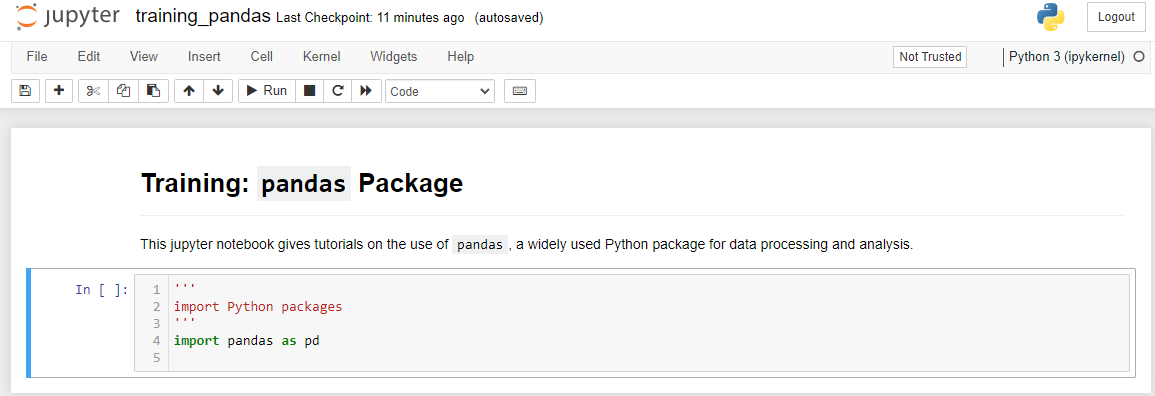
\includegraphics[width=350pt]{chapters/ch-python/figures/jupyter_cover.png}
	\caption{An example of a jupyter notebook.} \label{ch:python:fig:jupyter_cover}
\end{figure}


\section{Data Preprocessing}

Preprocessing of data is always required in data science. The format of data needs to be tidied, and error samples removed. Even with very clean input data, it is often necessary to do feature analysis and scaling (feature normalization). For verification of the effectiveness of the model to be built, data splitting into training set and testing set is often required.

Commonly used packages are imported as follows.
\begin{lstlisting}
import numpy as np
import matplotlib.pyplot as plt
import pandas as pd
\end{lstlisting}